\documentclass[12pt,a4paper]{article}
\usepackage[utf8]{inputenc}
%加這個就可以設定字體
\usepackage{fontspec}
%使用xeCJK,其他的還有CJK或是xCJK
\usepackage{xeCJK}
\usepackage{enumerate}
%設定英文字型,不設的話就會使用預設的字型
\usepackage{hyperref}
\usepackage{graphicx}
\usepackage{geometry}
\geometry{a4paper,scale=0.8}
\setmainfont{Times New Roman}
\usepackage{listings}
\lstset{language=python}
%設定中英文的字型
%字型的設定可以使用系統內的字型,而不用像以前一樣另外安裝
\setCJKmainfont{標楷體}
%以下是新增的自定义格式更改
\usepackage[]{caption2} %新增调用的宏包
\renewcommand{\figurename}{fig} %重定义编号前缀词
%中文自動換行
\XeTeXlinebreaklocale "zh"

%文字的彈性間距
\XeTeXlinebreakskip = 0pt plus 1pt

%設定段落之間的距離
\setlength{\parskip}{0.3cm}
\title{Neural Network Summary}
\author{虎尾科技大學\\40723115\\ 林于哲}
\date{January 16 2021}
\renewcommand{\contentsname}{目錄} %將content轉為目錄
\begin{document}
\maketitle
\tableofcontents

%摘要開始部分
\newpage
\begin{huge}\textbf{Introduction}\end{huge}\\
\begin{itemize}
\item Activation Function 
   \begin{enumerate}[I.]
   \item Sigmoid Function
   \item Relu
   \end{enumerate}
\end{itemize}   
\begin{itemize}
\item Optimizer
   \begin{enumerate}[I.]
   \item Adam
   \item SigmoidPrime
   \end{enumerate}
\end{itemize}  
\begin{itemize}   
\item Loss function
   \begin{enumerate}[I.]
   \item Mean Squared Error
   \end{enumerate}
\end{itemize} 


\section{Sigmoid Function}
An activation function.It is a key part of Nerual Network and it can be differentiable.It can make the Nenual Network unliner.\\
\begin{Large}$$\sigma(x)=\frac{1}{1+e^{-x}}$$ \end{Large}\\[6pt]
\begin{figure}[hbt!]
\begin{center}
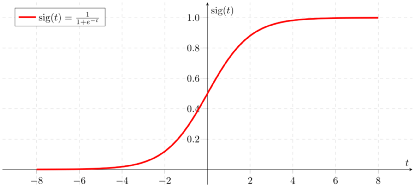
\includegraphics[scale=0.74]{sigmoid}
\caption{Sigmoid; from: \href{https://towardsdatascience.com/derivative-of-the-sigmoid-function-536880cf918e}{Toward Data Science}}
\end{center}
\end{figure}


\section{SigmoidPrime Function}
It is an differential Sigmoid Funtion. It can reduce  error of gradient so it is some kind of loss function and Let's take a look the proof of SigmoidPrime\\
\begin{Large}$$\sigma(x)=\frac{1}{1+e^{-x}}$$ \end{Large}\\[6pt]
$$\sigma^{'}(x)=\frac{d}{dx}\sigma(x)=\frac{d}{dx}\frac{1}{1+e^{-x}}=\frac{d}{dx}(1+e^{-x})^{-1}$$\\[6pt]
$$-------------skip-------------$$\\[6pt]
Tip: find $f^{'}(x)$ if $f(x)=\frac{A}{B+Ce^{x}}$\\
Answer:\\
$$\frac{d}{dx}[\frac{1}{g(x)}]=\frac{1^{'}g(x)-1g^{'}(x)}{g(x)^2}=\frac{g^{'}(x)}{[g(x)]^2}$$\\
if $g(x)$=constant\\
$$\frac{d}{dx}[\frac{g(x)}{h(x)}]=\frac{g^{'}(x)h(x)-g(x)h^{'}(x)}{h(x)^2}= \frac{-kh^{'}(x)}{[h(x)]^2}$$\\
$$f^{'}(x)=\frac{-A[\frac{d}{dx}(B+Ce^x)]}{(B+Ce^x)^2}=\frac{-A(0+Ce^x)}{(B+Ce^x)^2}=\frac{-ACe^x}{(B+Ce^x)^2}$$\\[6pt]
$$-------------skip-------------$$\\[6pt]
Hence:\\
$$=-(1+e^{-x})^{-2}\frac{d}{dx}(1+e^{-x})=-(1+e^{-x})^{-2}[\frac{d}{dx}(1)+\frac{d}{dx}(e^{-x})]$$\\
$$=-(1+e^{-x})^{-2}[0+\frac{d}{dx}(e^{-x})]=-(1+e^{-x})^{-2}[\frac{d}{dx}(e^{-x})]=-(1+e^{-x})^{-2}[e^{-x}\frac{d}{dx}(-x)]$$\\
$$-(1+e^{-x})^{-2}[e^{-x}(-1)]=-(1+e^{-x})^{-2}(-e^{-x})=\frac{e^{-x}}{(1+e^{-x})^2}=\frac{1(e^{-x})}{(1+e^{-x})(1+e^{-x})}$$\\
$$=\frac{1}{1+e^{-x}}\frac{e^{-x}}{1+e^{-x}}=\frac{1}{1+e^{-x}}\frac{e^{-x}+1-1}{1+e^{-x}}=\frac{1}{1+e^{-x}}(\frac{1+e^{-x}}{1+e^{-x}}-\frac{1}{1+e^{-x}})$$\\[6pt]
\begin{Large}$$=\sigma(x)[1-\sigma(x)]$$\end{Large}\\
\begin{figure}[hbt!]
\begin{center}
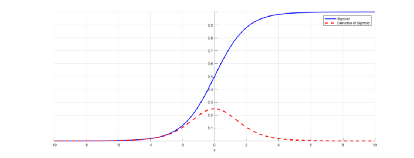
\includegraphics[scale=0.80]{sigmoidprime}
\caption{SigmoidPrime; from: \href{https://towardsdatascience.com/derivative-of-the-sigmoid-function-536880cf918e}{Toward Data Science}}
\end{center}
\end{figure}
\section{Relu Function}
This is the most commly used activation function in nerual network.It also can solve the Gradient Descent problem.
\begin{Large}$$f(x)=max(0,x)$$\end{Large}
$$if , x<0 , f(x)=0$$
$$else f(x)=x$$\\

\begin{figure}[hbt!]
\begin{center}
\includegraphics[height=4.5cm]{relu}\\
\caption{Relu; from : \href{https://www.kaggle.com/dansbecker/rectified-linear-units-relu-in-deep-learning}{\underline{kaggle}} 
}
\end{center} 
\end{figure}

\section{Adam Function}
Combine the advantage of Adagrad and RMSprop.The paper contained some very promising diagrams, showing huge performance gains in terms of speed of training but in some cases Adam actually finds worse solution than stochastic gradient descent. Let's take a look caculation prosess \\[6pt]
$$g_t=\delta_{\theta}f(\theta)$$\\
First moment exponentially moving averages : $m_t =\beta(m_{t-1})+(1-\beta_1)(\nabla{w_t})$\\[6pt]
$\hat m_t=\frac{m_t}{1-\beta_1^t}$\\[6pt]
Second moment exponentially moving averages :$v_t=\beta_2(v_t-1)+(1-\beta_2)(\nabla{w_t})^2$\\[6pt]
$\hat{v_t}=\frac{v_t}{1-\beta_2^t}$\\[6pt]
Hence,Adam Function:\\[6pt]
\begin{Large}$$\omega_{t-1}=\omega_t-\frac{\eta}{\sqrt{\hat{v_t}-\epsilon}}\hat{m_t}$$\end{Large}
\section{Mean Squared Error}
It tells you how close a regression lines to a set of points.It does this by taking the distances from the points to the regression line (these distances are the “errors”) and squaring them.The squaring is necessary to remove any negative signs. It also gives more weight to larger differences.(\href{https://www.statisticshowto.com/mean-squared-error/}{\underline{Extracted from here)}}.\\[6pt]

\begin{figure}
\center
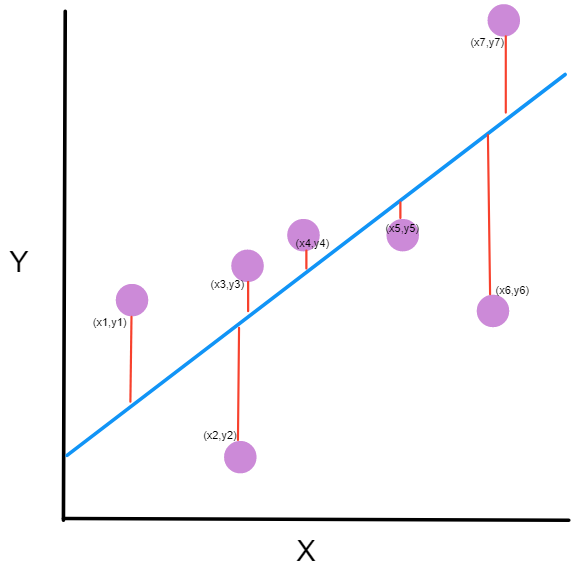
\includegraphics[height=7cm]{MSE}
\caption{regression line}
\end{figure}

regression line :It is a line of the minimize distance of data points. \\
n : number of data points\\
$y_i$ :  observed values\\
$\hat{y_i}$ : predicted values\\
\begin{Large}
$$MSE=\frac{1}{n} \sum_{i=1}^n(y_i-\overline{y} _i)^2$$
\end{Large}\\[6pt]



\section{Example Program}
This is XOR in nerual network program.
\href{https://www.notion.so/code-40723115-eac4c4cacdaa4ee38ecaa3275b4cac81}{\underline{Checkout in Notion}}.\\
%\newpage
\begin{Large}Two Layer Neural Network:\end{Large}
\begin{flushleft}
\begin{lstlisting}[language=python]
# numpy建構兩層的神經網路
import numpy as np
# X = input of our 3 input XOR gate
#X=輸入三個XOR gate值當作input
# set up the inputs of the neural network 
  (right from the table)
#設置神經網路的輸入
X = np.array(([0,0,0],[0,0,1],[0,1,0],/
[0,1,1],[1,0,0],[1,0,1],[1,1,0],[1,1,1]), dtype=float)
#建立輸入為一維的array,裡面元素型態為float
# y = our output of our neural network
#y= 神經網路的輸出
#建立輸出為一維的array,裡面元素類型為float
y = np.array(([1], [0], [0], 
[0], [0],[0], [0], [1]), dtype=float)
# what value we want to predict
#我們想預測的值
#建立預測值為一維的array,裡面元素類型維float
xPredicted=np.array(([0,0,1]),dtype=float)
# maximum of X input array # 一維X輸入數組或
最大數組通過axis指定為行
X = X/np.amax(X, axis=0) 
# maximum of xPredicted (our input datafor the prediction)
#最大的xPredicted(用於預測的輸入數據)
# 一維預測值或最大預測值,通過axis指定為行
xPredicted = xPredicte/np.amax(xPredicted, axis=0)
# set up our Loss file for graphing
#設置Loss file以作圖
#設置loss結果圖檔案為"SumSquaredLossList.csv"
lossFile = open("SumSquaredLossList.csv", "w")
#網路中每層的python代碼(物件導向)
#建立類別Neural_Network,屬性object
class Neural_Network (object):
#定義初始化物件的屬性值,並告訴類別目前是在設定哪一個物件的屬性
    def __init__(self):
        #parameters
#此物件的inputLayerSize屬性等於傳入的inputLayerSize屬性值
#隱藏層大小=3
# X1,X2,X3
        self.inputLayerSize = 3
# Y1 
#此物件的outputLayerSize屬性等於傳入的outputLayerSize屬性值 
#隱藏層大小=1
        self.outputLayerSize = 1 
# Size of the hidden layer
#此物件的hiddenLayerSize屬性等於傳入的hiddenLayerSize屬性值 
#隱藏層大小=4
        self.hiddenLayerSize = 4 
# build weights of each layer 
#建立每層的權重
# set to random values
 #將所有權重設置為隨機值,即為互聯圖
# look at the interconnection diagram to make sense of this
# 3x4 matrix for input to hidden #用於input到hidden layer的3X4矩陣
#權重#keras的kernel
        self.W1 = \
        np.random.randn\
        (self.inputLayerSize, self.hiddenLayerSize) #0,1
# 4x1 matrix for hidden layer to output 
#用於hidden layer到output的4x1矩陣
        self.W2 = \
        np.random.randn
        (self.hiddenLayerSize, self.outputLayerSize) #0,1
    def activationSigmoid(self, s):
# activation function
# simple activationSigmoid curve as in the book
        return 1 / (1 + np.exp(-s))#sigmoid函数

    def feedForward(self, X):#X放入函數
# feedForward propagation傳播 through our network
# dot product of X (input) and first set of 3x4 weights
#第一個設置的3x4權重和X(input)點積
        self.z = np.dot(X, self.W1)
# the activationSigmoid activation function - neural magic
        self.z2 = self.activationSigmoid(self.z)#激勵函數
# dot product of hidden layer (z2) and second set of 4x1 weights
        self.z3 = np.dot(self.z2, self.W2)
# final activation function - more neural magic
        o = self.activationSigmoid(self.z3)#激勵函數
        return o

    def activationSigmoidPrime(self, s):#修正斜率誤差
        # First derivative of activationSigmoid
        #activationSigmoid的倒數
        # calculus time!
        #微分時間
        return s * (1 - s)

    def backwardPropagate(self, X, y, o):
# backward propagate through the network
# calculate the error in output#計算output錯誤
#計算輸出誤差
        self.o_error = y - o 
# apply derivative of activationSigmoid to error
#應用activationSigmoidPrime於錯誤
        self.o_delta = self.o_error*self.activationSigmoidPrime(o)
# z2 error: how much our hidden layer weights contributed to output
# error
#多少的隱藏層權重到output
        self.z2_error = self.o_delta.dot(self.W2.T)#轉置矩陣
# applying derivative of activationSigmoid to z2 error
#將ActivationSigmoid的導數應用於z2錯誤
        self.z2_delta = 
        self.z2_error*self.activationSigmoidPrime(self.z2)
# adjusting first set (inputLayer --> hiddenLayer) weights
#調整第一組(輸入圖層->隱藏圖層)權重
        self.W1 += X.T.dot(self.z2_delta)
#adjusting second set (hiddenLayer --> outputLayer) weights
#調整第二組(隱藏層->輸出層)權重
        self.W2 += self.z2.T.dot(self.o_delta)
    
    def trainNetwork(self, X, y):
# feed forward the loop
#feed forward迴圈
        o = self.feedForward(X)
# and then back propagate the values (feedback)
#然後向後傳播值(反饋)
        self.backwardPropagate(X, y, o)
#將損失函數值保存到excel和神經網路權重文件中 
#\n 代表换行,print出来一个新行
    def saveSumSquaredLossList(self,i,error):
        lossFile.write(str(i)+","+str(error.tolist())+'\n')
        
    def saveWeights(self):
        # save this in order to reproduce our cool network
        np.savetxt("weightsLayer1.txt", self.W1, fmt="%s")
        #將self.W1反向存成txt檔,fmt="%s"導致數字格式化
        np.savetxt("weightsLayer2.txt", self.W2, fmt="%s")
        
    def predictOutput(self):
        print ("Predicted XOR output data based on 
        trained weights: ")
        print ("Expected (X1-X3): \n" + str(xPredicted))
        print ("Output (Y1): \n" +str(self.feedForward(xPredicted)))
myNeuralNetwork = Neural_Network()
trainingEpochs = 1000
#trainingEpochs = 1000
for i in range(trainingEpochs): 
# train myNeuralNetwork 1,000 times
    print ("Epoch # " + str(i) + "\n")
    print ("Network Input : \n" + str(X))
    print ("Expected Output of XOR Gate Neural Network: \n" 
    + str(y))
    print ("Actual Output from XOR Gate Neural Network: \n"
    + str(myNeuralNetwork.feedForward(X)))
    # mean sum squared loss
    #平均平方損失值
    Loss = np.mean(np.square(y - myNeuralNetwork.feedForward(X)))
    myNeuralNetwork.saveSumSquaredLossList(i,Loss)
    print ("Sum Squared Loss: \n" + str(Loss))
    print ("\n")
    myNeuralNetwork.trainNetwork(X, y)
myNeuralNetwork.saveWeights()
myNeuralNetwork.predictOutput()
\end{lstlisting}
\end{flushleft}

\begin{Large}XOR Tensorflow in Nerual Network:\end{Large}\\[6pt]
\begin{lstlisting}[language=python]
import tensorflow as tf

from tensorflow.keras import layers

from tensorflow.keras.layers import Activation, Dense

import numpy as np

# X = input of our 3 input XOR gate
# set up the inputs of the neural network (right from the table)
X = np.array(([0,0,0],[0,0,1],[0,1,0], 
            [0,1,1],[1,0,0],[1,0,1],[1,1,0],[1,1,1]), dtype=float)
# y = our output of our neural network
y  = np.array(([1], [0],  [0],  [0],  [0], 
             [0],  [0],  [1]), dtype=float)

#define-->compile-->fit-->evaluate-->make Predictions
model = tf.keras.Sequential()#多個網路層線性堆疊的序貫模型

model.add(Dense(4, input_dim=3, activation='relu',
use_bias=True))#Dense:output = 
activation(dot(input, kernel(權重矩陣))+bias)
#model.add(Dense(4,  activation='relu', use_bias=True))
model.add(Dense(1, activation='sigmoid', use_bias=True))

model.compile(loss='mean_squared_error',optimizer='adam',
metrics=['binary_accuracy'])
#loss:損失函數 optimizer:優化器 metrics:判定model的準確率(評
估);計算預測值與use_bias的符合頻率

print (model.get_weights())

history = model.fit(X, y, epochs=200, validation_data = (X, 
y))#modle.fit()用以訓練模型 ; validation_data:在每次訓練結束時,
評估損失數據和metrics值


model.summary()#method to display sequential contents


# printing out to file
#.history紀錄連續迭代的loss值
loss_history = history.history["loss"]

numpy_loss_history = np.array(loss_history)
np.savetxt("loss_history.txt", 
numpy_loss_history,delimiter="\n") #字串或字符的分隔列

binary_accuracy_history = 
history.history["binary_accuracy"]#.history紀錄連續迭代的metrics值
numpy_binary_accuracy = np.array(binary_accuracy_history)
np.savetxt("binary_accuracy.txt", numpy_binary_accuracy, 
delimiter="\n")
print(np.mean(history.history["binary_accuracy"],
dtype=np.float64))
#print出每次metrics的平均值

result = model.predict(X).round()#結果預測

print (result)
\end{lstlisting}
\end{document}  
